\chapter{Planificación}

\section{Metodología utilizada}

El software es un sistema complejo de crear que depende de muchas partes interconectadas. No es igual de dificultoso programar un pequeño \textit{script} que ordene los ficheros de un directorio de un sistema operativo que construir una aplicación de cierta envergadura que responda a las necesidades de un usuario o un cliente concreto, mucho más si además se debe coordinar un equipo de personas en la concepción del mismo. Existe un gran factor de riesgo e incertidumbre, sobre todo al inicio de un proyecto. Las \textbf{metodologías de desarrollo ágil} son una forma de desarrollar software enfocada a equipos pequeños que busca paliar estos problemas a la hora de encarar un proyecto,. En otras metodologías anteriores se redactaban unos requisitos completos y fijos al inicio del proyecto y antes si quiera de comenzar la implementación. Esto era una fuente común de conflictos, ya que es muy común que los requisitos cambien a lo largo del desarrollo. Quizás el cliente cambie de idea, o el equipo encuentre mejores formas de realizar una tarea, o el contexto en el ámbito en el que se desarrolla el producto ha cambiado y hay que adaptar ciertas partes del proyecto, etc. La incertidumbre es un elemento muy presente, y las metodologías ágiles la abraza. Conviven con el cambio inevitable estableciendo unas bases menos sólidas pero más flexibles. Esta forma de trabajar se enunció oficialmente por primera vez en 2001, en el documento de \textbf{Manifiesto Ágil}\footnote{El Manifiesto Ágil se puede consultar en esta web oficial. Hay una versión en español en la misma web. \url{https://agilemanifesto.org/}}. Esta forma de organizar proyectos  se fundamenta en cuatro puntos, extraidos del libro \textit{Métodos Ágiles y Scrum}\cite{agilescrum}:

\begin{itemize}
    \item \textbf{Valorar a individuos y sus interacciones}, frente a procesos y herramientas. Aunque todas las ayudas para desarrollar un trabajo son importantes, nada sustituye a las personas, a las que hay que dar toda la importancia y poner en primer plano.
    \item \textbf{Valorar más el software (producto) que funciona}, que una documentación exhaustiva. Porque había llegado un punto en el que documentar el trabajo había alcanzado tanta importancia como el objeto del trabajo: el producto.
    \item \textbf{Valorar más la colaboración con el cliente} que la negociación de un contrato. La forma más productiva de sacar adelante un trabajo es establecer un marco de confianza y colaboración con quien nos lo encarga. Sin embargo se estaba poniendo el foco en cerrar un contrato atado que sirviera ante todo como una herramienta de protección, como si el cliente y equipo fueran dos partes enfrentadas, cuando en realidad comparten objetivos e intereses.
    \item \textbf{Valorar más la respuesta al cambio} que el seguimiento de un plan. Se trata de apreciar la incertidumbre como un componente básico del trabajo, por lo que la adaptación y la flexibilidad se convierten en virtudes y no en amenazas. El seguimiento ciego de un plan lleva, salvo contadas excepciones, al fracaso si no se puede corregir la dirección ante los inevitables cambios que van surgiendo.
\end{itemize}

Este típo de metodologías intentan aplicar un cambio de paradigma: mientras que tradicionalmente se fijaban unos requisitos a partir de los cuales se estimaban los recursos y plazos que se requerirían para su terminación, la forma ágil sería fijar unos recursos y fechas disponibles en las que se disponen para el trabajo, y a partir de ahí estimar los requisitos que va a tener el producto al final. Se eligió optar por esta forma de encarar proyectos ya que en primer lugar el trabajo tenía una fecha de finalización fíja, y además no se tenía experiencia en algunos de los campos requeridos para el desarrollo, como podría ser por ejemplo la implementación de interfaces web. Se iba a requerir de un periodo de formación paralela al desarrollo, lo cual con total probabilidad cambiará la visión del desarrollador sobre la estimación de los costes y tiempo del proyecto. Sería contraproducente espablecer desde un inicio unos requisitos fijos si se prevé que van a cambiar, y  las metodologías ágiles se ajustaban perfectamente a este escenario.

Una vez definidos los métodos de desarrollo ágil y entendido por qué son convenientes para este proyecto en particular, se debe elegir uno de los que hay disponibles como \textit{Lean Software Development}, \textit{Kanban}, \textit{Pragmatic Programming} o \textit{eXtreme Programming}. En este caso se ha optado por \textbf{SCRUM}\cite{scrum}, una de las metodologías más difundidas.

\textit{SCRUM} proporciona un marco de trabajo para equipos de desarrollo pequeños y autogestionados. Como en este caso el trabajo se realiza de forma individual los roles que propone este método se han sintetizado en una sola persona. Originalmente se tenía al equipo de desarrollo, el \textit{Product Owner} (dueño del producto o cliente) y el \textit{SCRUM Master}, el encargado de que el equipo sea efectivo.

Se trabaja definiendo una serie de \textit{sprints}, iteraciones de dos semanas de duración las cuales deben presentar un producto entregable al final de cada una, como por ejemplo un software ejecutable. Al comienzo de cada  sprint se hace el \textit{sprint planning}, una reunión en la que se planifica el trabajo a desarrollar durante la iteración. Al final de cada sprint se realiza el \textit{sprint review} en el que se valora cómo se ha trabajado y qué aspectos mejorar para el siguiente sprint. Las \textit{daily meetings} que propone SCRUM en las que cada miembro del equipo comenta en qué estado del trabajo se encuentra se ha omitido para este proyecto por ser solo un integrante en el equipo.

\section{Historias de usuario}

Para describir los requisitos del sistema a desarrollar se emplearán \textit{historias de usuario}. Estas son descripciones del sistema que se usan para plasmar los requisitos del mismo desde el punto de vista del usuario. Se redactan al comienzo del desarrollo, durante el \textit{Sprint 0} del que se hablará más adelante, y a partir de estas se redactan las \textit{tareas} del desarrollo.

Antes de redactar las historias es necesario definir definir los distintos perfiles que van a hacer uso del producto. En este caso se tiene un único perfil:

\begin{itemize}
    \item \textbf{Usuario}: Este perfil representa a un consumidor casual, que puede o no tener nociones tanto de Realidad Aumentada como de modelado 3D. Tiene una experiencia como poco básica en el manejo de ordenadores y aplicaciones de los mismos, usando tanto el teclado como el ratón para interactuar con distintos elementos en pantalla. Es usuario de servicios como correo electrónico y está familiarizado con el proceso de iniciar sesión con contraseña. Tiene los recursos para poder encontrar en internet modelos 3D gratuitos y descargarlos en su equipo.
\end{itemize}

Una vez definido el perfil que hará uso del software se redactarán los \textit{journeys}. Estas son una descripción en forma de narración en la que se detalla el uso que un usuario concreto (que no un perfil de usuario) hace uso del producto desde el inicio hasta al final. Esto servirá para comprender mejor las necesidades de estos y reflejarlas en las historias de usuarios.

\begin{itemize}
    \item \textbf{J-01}: Florentino Pérez es un hombre de 42 años. Escucha sobre la tecnología de Realidad Aumentada en el telediario y le parece de lo más vistosa e innovadora, por lo que suscita su curiosidad y decide probarla. Tras una breve búsqueda en Google encuentra EditAR entre otras opciones, y decirle probarla porque aparenta ser sencilla. Tras acceder a la web sigue las instrucciones para registrarse como usuario. Una vez hecho, selecciona la opción de crear escena, y empieza a componer una del tipo de posicionamiento en superficies. Carga modelos 3D que ha encontrado en una web de recursos gratuitos y hace click en ellos para manipularlos y colocarlos donde él prefiera. Cuando ha terminado selecciona la opción de guardar la escena. Florentino procede a instalar en su dispositivo móvil la aplicación del visor. En ella inicia sesión con las credenciales que introdujo en pasos anteriores. Aparece un menú con la única escena que ha creado y selecciona la opción de reproducir. Se inicia la cámara de su dispositivo y procede a colocar el modelo de la escena encima de su escritorio. Florentino observa cómo detecta la superficie y coloca el objeto. Incluso aunque mueva la cámara de ángulo sigue dando la sensación de que el objeto está en la mesa. Satisfecho, cierra la aplicación.
    
    \item \textbf{J-02}: Belkan Díaz es un hombre de unos 20 años. Acaba de adquirir un nuevo y flamante smartphone Xiaomi y está oteando la tienda de aplicaciones para descargar algunas para estrenarlo. De casualidad se topa con la aplicación de EditAR y acaba descubriendo también su web, así que decide probarla. Se registra en el sistema con sus credenciales y pasa a crear una escena de imágenes aumentadas con modelos 3D gratuitos de internet. Cuando ha terminado y la guarda, se da cuenta de que por error se ha registrado con el correo electrónico de su trabajo, lo cual es inapropiado, así que accede al menú de cambio de credenciales, e introduciendo su contraseña logra cambiar su dirección de email. Una vez solucionado eso, accede usando su nuevo correo desde la aplicación móvil y consigue reproducir la escena. Aunque le sorprende el funcionamiento de la realidad aumentada, no le gusta la escena que ha creado para nada, así que vuelve al editor para eliminarla y crear una nueva, la cual sí le convence.

    \item \textbf{J-03}: Antonia Miyamoto es una artista de modelos 3D. Tras haber oido hablar de la aplicación decide probarla con alguno de los modelos que ella misma ha diseñado. Accede a la web y se registra con sus credenciales. Piensa en que le gustaría ver un dragón sobrevolando su casa, así que inicia una nueva escena y la configura para que sea de tipo geoespacial. Introduce las coordenadas y altura de su vivienda, que ha podido obtener en algún servicio como \textit{Google Earth}. Carga el modelo del dragón que modeló días anteriores en \textit{Blender}. Lo coloca en la escena y selecciona que quiere que se reproduzca una animacioń del modelo en la que el dragón bate sus alas, para que de la sensación de que verdaderamente está volando. Una vez se da por satisfecha guarda la escena y cierra el editor. Instala la aplicación móvil e inicia sesión. Selecciona su escena y ve al dragón volando. Al verlo, piensa que podría quedar mucho mejor si mete una gran bola de fuego y una pista de audio de un gruñido de dragón. Antonia vuelve a abrir el editor y selecciona la escena que ya había creado en una opción que le permite editarla. El editor carga la escena tal como la dejó, lo que le permite añadir nuevos modelos para añadirle fuego. Además carga un archivo mp3 con el rugido. Cuando ve la nueva escena en su dispositivo móvil piensa que la escena ha quedado verdaderamente vistosa, y le gustaría exportarla para usarla en alguno de sus proyectos de \textit{Blender}, así que vuelve a abrir el editor web con la escena creada y hace click en un botoń que le exporta su escena y la descarga a su ordenador en forma de modelo 3D.
\end{itemize}

Una vez entendidas mejor las necesidades que tendrá el usuario del sistema se pueden redactar las historias de usuario. Para cada historia se definen una id que servirá para identificarla con formato \textbf{RA-X}, una descripción, unos requisitos asociados con formato \textbf{RF/RNF-X.n} y una prioridad. La prioridad podrá ser \textit{high} (alta) si describen elementos imprescindibles para el correcto funcionamiento del software y el cumplimiento de su propósito, \textit{mid} (media) si son de gran importancia pero la ausencia de alguna no es un impedimento crítico para el producto final, y \textit{low} para las historias que describen elementos preferibles, que aportan valor añadido pero que no son necesarios.

\subsection{RA-01: Entorno 3D}
Como usuario quiero tener un entorno 3D interactivo para configurar mis escenas de Realidad Aumentada.

\begin{itemize}
    \item Prioridad: \textbf{HIGH}
    \item Requisitos: Ninguno
\end{itemize}

\subsection{RA-02.1: Escenas de superficie}
Como usuario la posibilidad de crear escenas de Realidad Aumentada de posicionamiento por superficies.

\begin{itemize}
    \item Prioridad: \textbf{HIGH}
    \item Requisitos: Ninguno
\end{itemize}

\subsection{RA-02.2: Escenas de imágenes aumentadas}
Como usuario la posibilidad de crear escenas de Realidad Aumentada de imágenes aumentadas.

\begin{itemize}
    \item Prioridad: \textbf{HIGH}
    \item Requisitos: Ninguno
\end{itemize}

\subsection{RA-02.3: Escenas geoespaciales}
Como usuario la posibilidad de crear escenas de Realidad Aumentada geoespaciales introduciendo una latitud, longitud y altura concreta.

\begin{itemize}
    \item Prioridad: \textbf{HIGH}
    \item Requisitos: Ninguno
\end{itemize}

\subsection{RA-03: Varias imágenes activadoras}
Como usuario quiero, al crear una escena por marcador, poder definir varias imágenes activadoras, y distintos modelos asociados a cada una de ellas.

\begin{itemize}
    \item Prioridad: \textbf{LOW}
    \item Requisitos: Ninguno
\end{itemize}

\subsection{RA-04: Animaciones}
Como usuario quiero que los modelos que cargo puedan tener animaciones, y decidir si se reproducen al ver la escena una vez, en bucle o no lo hacen.

\begin{itemize}
    \item Prioridad: \textbf{MID}
    \item Requisitos: Ninguno
\end{itemize}

\subsection{RA-05: Pistas de audio}
Como usuario quiero poder cargar audios que se reproduzcan cuando se dispara la escena, y decidir si se reproducen una vez o en bucle.

\begin{itemize}
    \item Prioridad: \textbf{MID}
    \item Requisitos:
            \begin{itemize}
                \item \textbf{RF-5.1}: Cada escena tendrá asociado un único audio como mucho.
            \end{itemize}
\end{itemize}

\subsection{RA-06: Carga de modelos}
Como usuario quiero cargar un modelo 3D desde mi ordenador para añadirlo a la escena, así como eliminarlo más adelante.

\begin{itemize}
    \item Prioridad: \textbf{HIGH}
    \item Requisitos:
            \begin{itemize}
                \item \textbf{RNF-6.1}: Los modelos cargados deben ser de formato GLB con las restricciones para su uso en Filament.
            \end{itemize}
\end{itemize}

\subsection{RA-07: Transformaciones}
Como usuario quiero poder seleccionar un objeto 3D de la escena haciendo click sobre él y poder moverlo, rotarlo o hacerlo más grande o más pequeño.
\begin{itemize}
    \item Prioridad: \textbf{HIGH}
    \item Requisitos: Ninguno
\end{itemize}

\subsection{RA-08: Selección múltiple}
Como usuario quiero poder seleccionar más de un objeto a la vez para poder aplicarles los mismos cambios como moverlos, rotarlos o cambiarlos de tamaño.

\begin{itemize}
    \item Prioridad: \textbf{LOW}
    \item Requisitos: Ninguno
\end{itemize}

\subsection{RA-09: Figuras básicas}
Como usuario quiero poder crear figuras geométricas básicas como esferas, cubos, pirámides o cilindros entre otras.

\begin{itemize}
    \item Prioridad: \textbf{LOW}
    \item Requisitos: Ninguno
\end{itemize}

\subsection{RA-09.1: Texturas}
Como usuario quiero un menú en el que poder cambiar el color de las figuras básicas que creo.

\begin{itemize}
    \item Prioridad: \textbf{LOW}
    \item Requisitos: Ninguno
\end{itemize}

\subsection{RA-10: Inicio de sesión}
Como usuario quiero poder iniciar sesión con mis datos en la aplicación web para que, si accedo desde otro ordenador, pueda recuperar datos mios como las escenas creadas.

\begin{itemize}
    \item Prioridad: \textbf{HIGH}
    \item Requisitos:
        \begin{itemize}
            \item \textbf{RNF-10.1}: Se almacenará y empleará para el inicio de sesión únicamenet el email y contraseña del usuario
        \end{itemize}
\end{itemize}

\subsection{RA-10.1: Cambio de credenciales}
Como usuario quiero tener la opción de modificar mi correo electrónico o contraseña en un futuro.

\begin{itemize}
    \item Prioridad: \textbf{MID}
    \item Requisitos: Ninguno
\end{itemize}

\subsection{RA-10.2: Guardado de escenas}
Como usuario quiero poder guardar bajo mi cuenta de usuario las escenas que creo para poder volver a abrirlas en un futuro y editarlas.

\begin{itemize}
    \item Prioridad: \textbf{HIGH}
    \item Requisitos: Ninguno
\end{itemize}

\subsection{RA-11.1: Reproducción de imágenes aumentadas}
Como usuario quiero poder reproducir en una app móvil en la que reproducir mis escenas de imágenes aumentadas, detectando con la cámara del teléfono la imagen que establecí en el editor como disparador de la escena.

\begin{itemize}
    \item Prioridad: \textbf{HIGH}
    \item Requisitos: Ninguno
\end{itemize}

\subsection{RA-11.2: Reproducción de escenas por superficies}
Como usuario quiero poder reproducir en una app móvil en la que reproducir mis escenas por superficies, las cuales podré colocar en sitios como mesas o suelos. 

\begin{itemize}
    \item Prioridad: \textbf{HIGH}
    \item Requisitos: Ninguno
\end{itemize}

\subsection{RA-11.3: Reproducción de escenas geoespaciales}
Como usuario quiero poder reproducir en una app móvil en la que reproducir mis escenas geoespaciales, en las cuales podré ver los modelos solo si estoy cerca de ciertas coordenadas que introduje en el editor a la hora de crear la escena.

\begin{itemize}
    \item Prioridad: \textbf{MID}
    \item Requisitos: Ninguno
\end{itemize}

\subsection{RA-12: Inicio de sesión en la app móvil}
Como usuario quiero iniciar sesión en la app móvil para acceder a las escenas que previamente he creado

\begin{itemize}
    \item Prioridad: \textbf{HIGH}
    \item Requisitos: Ninguno
\end{itemize}

\subsection{RA-12.1: Listado de escenas}
Como usuario quiero tener en la app móvil un listado de todas las escenas que he creado para poder seleccionarla y reproducirla.

\begin{itemize}
    \item Prioridad: \textbf{MID}
    \item Requisitos: Ninguno
\end{itemize}

\subsection{RA-12.1: Filtrado de escenas}
Como usuario quiero en el listado de escenas poder filtrarlas por tipo o por nombre, para poder encontrar la que me interesa rápidamente.

\begin{itemize}
    \item Prioridad: \textbf{LOW}
    \item Requisitos: Ninguno
\end{itemize}

\subsection{RA-13: Exportación de escenas}
Como usuario quiero poder exportar mi escena y modelos a un formato que permita ser utilizado por aplicaciones móviles de realidad aumentada.

\begin{itemize}
    \item Prioridad: \textbf{HIGH}
    \item Requisitos:
        \begin{itemize}
            \item \textbf{RNF-13.1}: Las escenas con varios modelos cargados deben exportarse como un solo modelo.
        \end{itemize}
\end{itemize}

\section{Sprint 0}

El sprint 0 tiene la el objetivo de definir todo el trabajo que se va a realizar y cómo. Se estudia el problema para saber si es viable construir una solución. Esta iteración especial tuvo una duración de una semana. Aquí se realizaron las labores de investigación que se ha persebntado en los capítulo 2 y 3 de este trabajo. También se crea el \textit{product backlog}, la lista de historias de usuario que recoge la visión de los requisitos principales de la aplicación desde la perspectiva de sus usuarios que ya se redactó en el apartado anterior.

Otra actividad esencial de esta etapa es la definición y temporicación de los sprints que se desarrollarán en todo el desarrollo. Se decidió establecer un total de \textbf{cinco sprints de dos semanas cada uno} (sin incluir este). Las historias de usuario se dividirían entre los distintos sprints. Para cuando acaben cada uno de ellos, debe resultar una versión entregable del producto que implemente las funcionalidades y requisitos especificados por sus historias de usuario. Para ello, de cada historia de usuario se extraerá al principio de cada sprint una serie de \textbf{tareas} que completar para avanzar el desarrollo. Se dividieron las historias de tal forma que las que se encasillen en un mismo sprint, guarden cierta relación entre ellas tematizando así las labores que se desarrollan en cada iteración. También se tuvieron en cuenta la prioridad de las historias, dejando la mayoría de las menos relevantes para sprints finales, por si hubiera complicaciones en alguno de los anteriores, priorizar las funcionalidades más esenciales.

\begin{figure}[h]
    \centering
    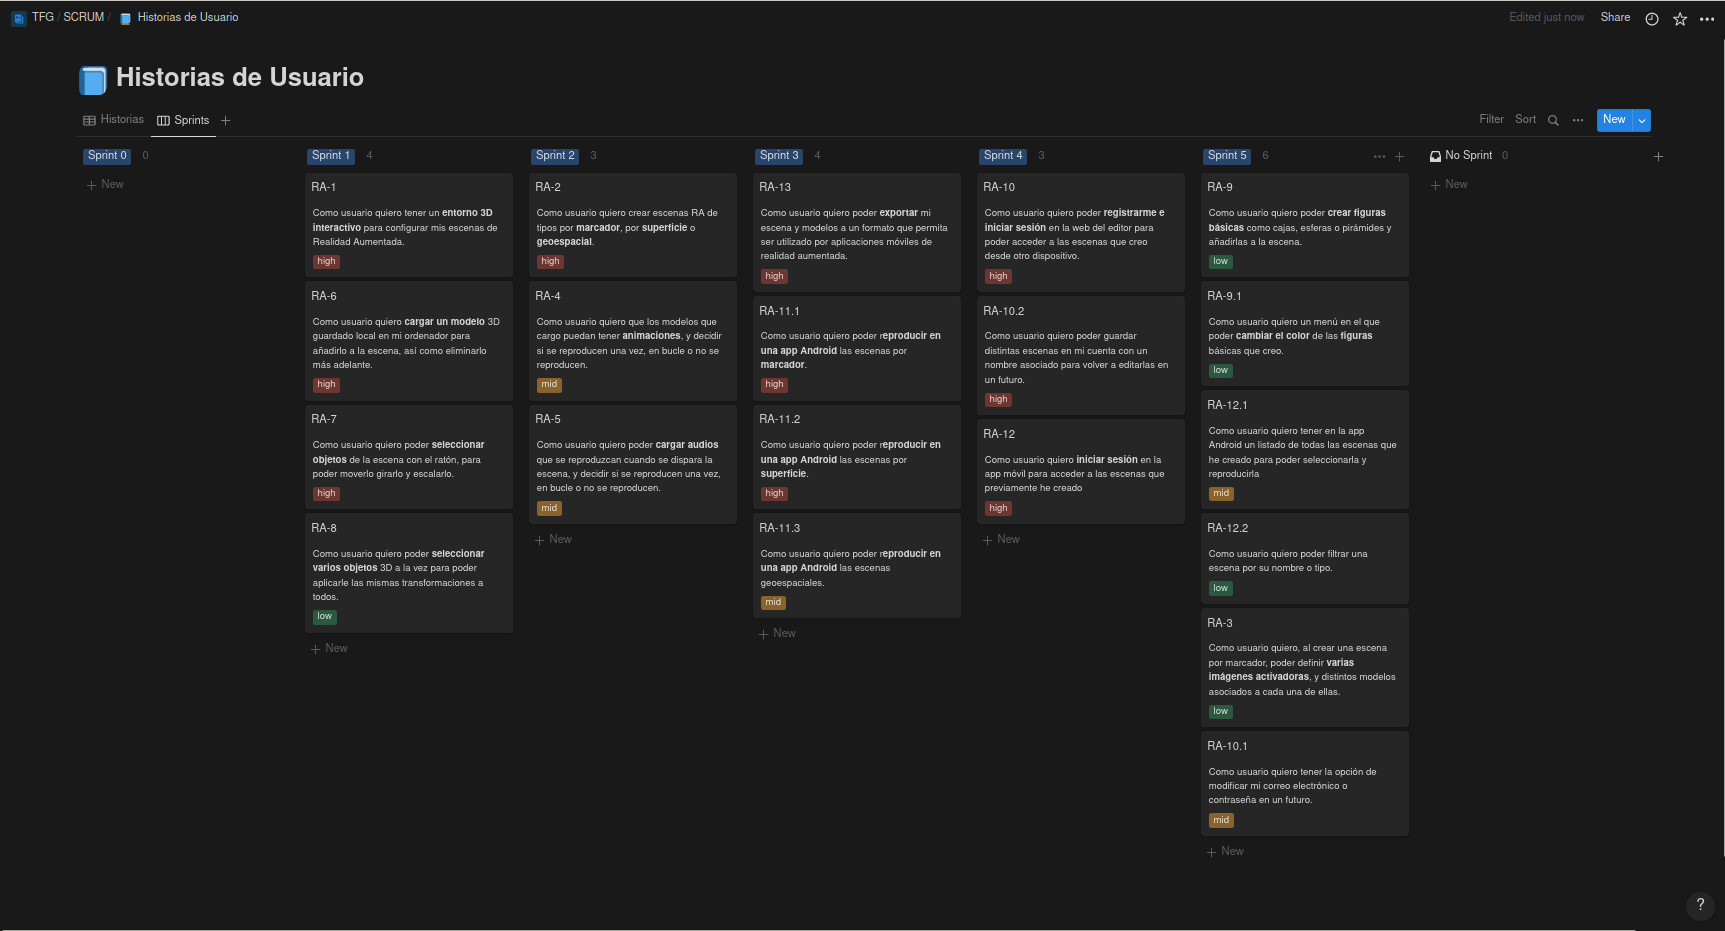
\includegraphics[scale=0.30]{sprinthu}
    \caption[Planificación de HU por sprints]{Distribución de las historias de usuario por sprints}
\end{figure}

Se definió también la temporización de estos sprints, comenzando el desarrollo el 17 de abril de 2023 y finalizando el 25 de junio de 2023:
\begin{itemize}
    \item \textbf{Sprint 1}: 17/4/23 a 30/4/23
    \item \textbf{Sprint 2}: 1/5/23 a 14/5/23
    \item \textbf{Sprint 3}: 15/5/23 a 28/5/23
    \item \textbf{Sprint 4}: 29/5/23 a 11/6/23
    \item \textbf{Sprint 5}: 12/6/23 a 25/6/23
\end{itemize}

Para cada sprint se tendrá un tablero de tareas en el que de un vistazo el desarrollador podrá obtener una idea de en qué estado del desarrollo se encuentra. Para ello se organizará la tabla en columnas, bajo las que se colocarán las distintas tareas según su estado, que pueden ser:

\begin{itemize}
    \item \textbf{Backlog}: Listado de tareas por implementar en el sprint
    \item \textbf{Implementación}: Las tareas que están en proceso de implementación en este momento.
    \item \textbf{Terminada}: Tareas finalizadas por completo.
    \item \textbf{Diseño}: Tareas que están en fase de diseño porque requieren de la elaboración de diagramas o similares.
    \item \textbf{Investigación}: Lista de tareas que requieren alguna labor de investigación adicional que no se había previsto.
    \item \textbf{Bloqueado}: Tareas que no pueden ser implementadas hasta que finalicen otras o que se han descartado por alguna razón.
\end{itemize}

\begin{figure}[h]
    \centering
    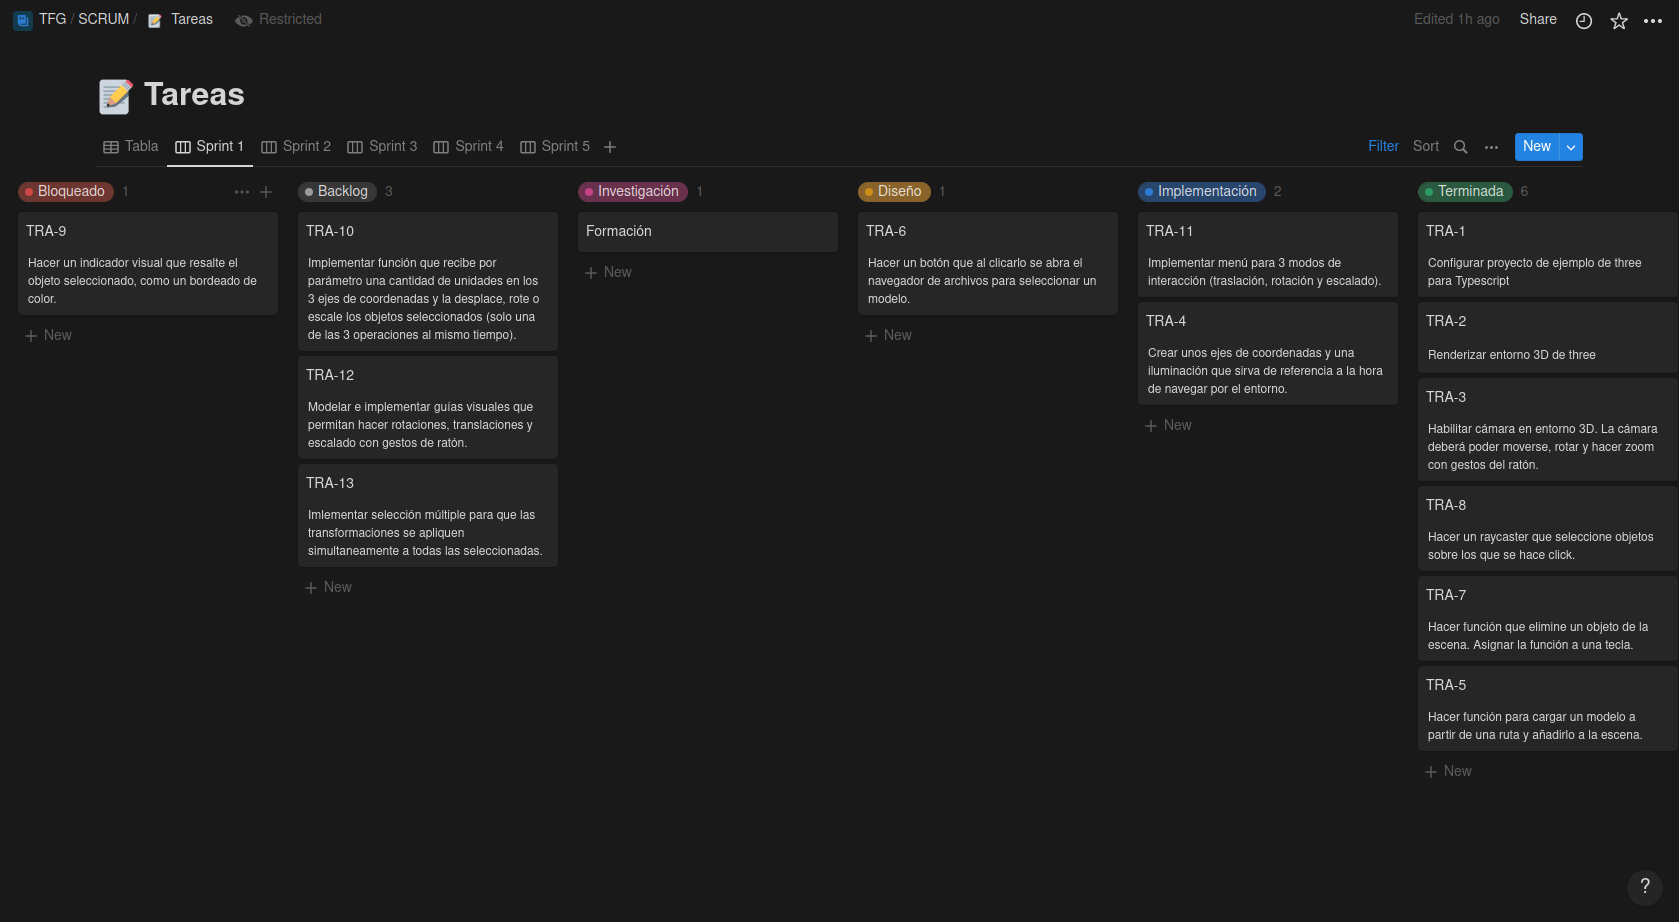
\includegraphics[scale=0.30]{tablero}
    \caption[Tabla de sprint]{Ejemplo de tabla para el sprint 1}
\end{figure}

Otra tarea esencial del sprint 0 es definir las tecnologías y herramientas que se usarán para el desarrollo para tener una visión más amplia del producto final y reducir la incertidumbre del desarrollo, por lo que es lo que se va a proceder a describir.

Como software de gestión de proyecto se optó por usar Notion\cite{notion}. Aquí se gestiona todo lo relacionado con la planificación del trabajo: historias, tareas, sprints, requisitos, tableros, etc. Se contemplaron otras opciones, principalmente \textit{Jira}\cite{jira}, pero era una herramienta demasiado compleja ya que está contemplada para el trabajo en equipo y en este caso el desarrollador era una única persona, por lo que era un software que venía demasiado grande para el propósito. Notion por otro lado, aunque no esté directamente diseñado para estos porpósitos, permite la creación de tablas, bases de datos y tableros, hiperenlaces a distintos documentos dentro de un espacio de trabajo y almacenamiento en la nube. Como software de gestión de proyectos se empleó \textit{Git y GitHub}, ya que es la plataforma más utilizada y con la que se contaba experiencia previamente, tenía todas las funcionalidades que se requerían para el proyecto. Se creó un repositorio\footnote{\url{https://github.com/pabloMillanCb/tfg}} público desde el primer momento con el proyecto íntegro publicado bajo licencia de software libre.

En cuanto a desarrollar aplicaciones web se refiere, \textit{JavaScript} es la única opción existente en cuanto a lenguajes ya que es el único que pueden ejecutar todos los navegadores, así que no hubo muchas dudas en ese aspecto. Aunque no se optó exactamente por \textit{JavaScript}, si no por \textit{TypeScript}, una extensión sintáctica para el lenguaje que añade la opción de introducir tipado estático a los objetos. Se tomó esta decisión porque se consideró que a cambio de invertir un poco más de tiempo en escribir el código, se podría ahorrar tiempo de depuración. Esto es posible ya que gracias a declarar los tipos de las variables, el editor puede detectar errores antes incluso de la ejecución, como por ejemplo intentar añadir un objeto \textit{String} a un array de objetos \textit{Object 3D}, evitándose así sorpresas desagradables en la ejecución.

Como se pretende desarrollar un editor que muestre y trabaje con modelos 3D, se necesitará un motor de gráficos por ordenador operable desde \textit{JavaScript} y con soporte para web. Las dos opciones que se tuvieron en cuenta fueron \textit{Three.js}\cite{three} y \textit{Babylon.js}\cite{babylon}, dos librerías \textit{JavaScript} para la renderización de gráficos 3D. Se optó por coger la primera, ya que tras analizar ambas no se encontró ninguna ventaja significative de una respecto a otra, y para \textit{Three.js} se contaba ya con experiencia, lo que aceleraría el desarrollo.

Para construir la aplicación web se barajaron dos opciones: \textit{Angular}\cite{angular}, un framework completo para \textit{JS} para el desarrollo de web y móvil o \textit{React.js}\cite{react}, una librería \textit{JS} para el desarrollo frontend. Se escogió esta última ya que, aunque \textit{Angular} es más completo y no necesita librerías externas para realizar ciertas funcionalidades, React es mucho más simple e intuitivo. Su curva de aprendizaje es mucho menos pronunciada, casi inmediata si se tiene conocimiento en \textit{JavaScript} como era el caso. Como no se tenía experiencia en ninguna de las dos herramientas, se optó por esta para reducir el periodo de formación requerido.

Para el visor de las escenas en móvil se decidió hacer una aplicación Android. Se es consciente de el hecho que supone una desventaja respecto a la versión web de otras opciones del mercado ya que en dispositivos iOS no funcionaría, pero se decidió apostar por una aplicación nativa ya que no la ofrece nuinguna otra propuesta. Se escogió Android porque es la plataforma mayoritaria en el mercado móvil. Para el desarrollo de la aplicación se escogió usar \textit{Android Studio} frente a \textit{React Native}. Ambos permiten escribir aplicaciones nativas, pero la primera tiene una mayor integración con \textit{Sceneview}, la librería escogida para las funcionalidades de Realidad Aumentada. Se programará en Kotlin en lugar de Java, ya que es la recomendación oficial de Google y la forma más moderna de hacerlo.

Para las funcionalidades de Realidad Aumentada se optó por ARCore\cite{arcore}, el SDK de Google para esta tecnología. El único problema que se presentaba con esta decisión es que ARCore renderiza objetos 3D a través de OpenGL, una API de bajo nivel que ralentizaría bastante el deasrrollo. Para paliarlo se adoptó Sceneview\cite{sceneview}, una librería para Kotlin que envuelve a ARCore y hace el renderizado mucho más simple.

Para las necesidades del proyecto era evidente que haría falta algún tipo de base de datos para almacenar información como los usuarios, las escenas de estos y los recursos como modelos y audio que componen las escenas. Era necesario desarrollar una API REST, una interfaz que emplean dos sistemas informáticos para intercambiar información de manera segura a través de la web. Para ello se pensó en un primer momento hacerla con PHP y MYSQL, pero finalmente se decidió usar \textit{Firebase}\cite{firebase}. Esta herramienta viene con muchas utilidades ya implementadas para que el desarrollador pueda hacer uso de estas con llamadas simples a su API, además de no invertir tiempo extra de desarrollo. Trae incorporado un servicio para el registro e inicio de sesión de usuarios \textbf{con contraseña encriptada} de forma automática, almacenamiento para archivos binarios y una base de datos no relacional entre otros. Para lo sencillo que se previó que iba a ser la infraestructura del backend (solo se necesitarían tablas para usuarios y escenas, además de una forma de guardar binarios en la base de datos) era una opción perfecta que se acomodaba a las necesidades y reducía mucho la complejidad del desarrollo.

Si bien Firebase ofrece todos esos servicios, seguía haciendo falta una API que lo comunicara con los clientes web y Android. Se decidió usar \textit{Node.js}\cite{nodejs} junto a \textit{Express}\cite{express}, ya que es una dupla ampliamente usada para el desarrollo de aplicaciones con Firebase con muchos recursos disponibles en internet. Además, no habría que familiarizarse con lenguajes nuevos, pues se programaría en \textit{JavaScript}

\section{Sprint 1}

Para este sprint se centraron esfuerzos en desarrollar las funcionalidades básicas del editor. El objetivo era que al final del sprint se tuviera un entorno 3D con una cámara la cual pudieras mover y rotar con el ratón, que hubieran varios objetos de prueba que fueran seleccionables con un click del ratón, además de la opción de cargar modelos. También se podrían aplicar transformaciones a través de un menú. Para realizar todo esto se añadieron al sprint la RA-01, RA-06, RA-07 y RA-08. De cada historia se extrae un backlog de tareas que se detalla a continuación.

\begin{table}[H]
	\resizebox{\textwidth}{!}{%
		\begin{tabular}{|l|l|l|l|l|}
			\hline
			\rowcolor[HTML]{EFEFEF} 
			\textbf{Tarea: TRA-01}           & \textbf{Horas estimadas: 3}      & \textbf{Horas totales: 1}            & \multicolumn{2}{l|}{\cellcolor[HTML]{EFEFEF}\textbf{HU asociada: RA-01}} \\ \hline
			\multicolumn{5}{|l|}{Configurar proyecto de ejemplo en Three.js con TypeScript}                   \\ \hline
		\end{tabular}%|m{15cm}
	}
\label{TRA-01}
\end{table}

\begin{table}[H]
	\resizebox{\textwidth}{!}{%
		\begin{tabular}{|l|l|l|l|l|}
			\hline
			\rowcolor[HTML]{EFEFEF} 
			\textbf{Tarea: TRA-02}           & \textbf{Horas estimadas: 1}      & \textbf{Horas totales: 1}            & \multicolumn{2}{l|}{\cellcolor[HTML]{EFEFEF}\textbf{HU asociada: RA-01}} \\ \hline
			\multicolumn{5}{|l|}{Renderizar entorno 3D de Three.js}                   \\ \hline
		\end{tabular}%|m{15cm}
	}
\label{TRA-03}
\end{table}

\begin{table}[H]
	\resizebox{\textwidth}{!}{%
		\begin{tabular}{|l|l|l|l|l|}
			\hline
			\rowcolor[HTML]{EFEFEF} 
			\textbf{Tarea: TRA-03}           & \textbf{Horas estimadas: 2}      & \textbf{Horas totales: 2}            & \multicolumn{2}{l|}{\cellcolor[HTML]{EFEFEF}\textbf{HU asociada: RA-01}} \\ \hline
			\multicolumn{5}{|l|}{\parbox{12cm}{Habilitar cámara en entorno 3D. La cámara deberá poder moverse, rotar y hacer zoom con gestos del ratón.}}                   \\ \hline
		\end{tabular}%|m{15cm}
	}
\label{TRA-03}
\end{table}

\begin{table}[H]
	\resizebox{\textwidth}{!}{%
		\begin{tabular}{|l|l|l|l|l|}
			\hline
			\rowcolor[HTML]{EFEFEF} 
			\textbf{Tarea: TRA-04}           & \textbf{Horas estimadas: 3}      & \textbf{Horas totales: 0.5}            & \multicolumn{2}{l|}{\cellcolor[HTML]{EFEFEF}\textbf{HU asociada: RA-01}} \\ \hline
			\multicolumn{5}{|l|}{\parbox{12cm}{Crear unos ejes de coordenadas y una iluminación que sirva de referencia a la hora de navegar por el entorno.}}                   \\ \hline
		\end{tabular}%|m{15cm}
	}
\label{TRA-04}
\end{table}

\begin{table}[H]
	\resizebox{\textwidth}{!}{%
		\begin{tabular}{|l|l|l|l|l|}
			\hline
			\rowcolor[HTML]{EFEFEF} 
			\textbf{Tarea: TRA-05}           & \textbf{Horas estimadas: 1}      & \textbf{Horas totales: 0.1}            & \multicolumn{2}{l|}{\cellcolor[HTML]{EFEFEF}\textbf{HU asociada: RA-06}} \\ \hline
			\multicolumn{5}{|l|}{\parbox{12cm}{Hacer una función para cargar un modelo a partir de una ruta y añadirlo a la escena.}}                   \\ \hline
		\end{tabular}%|m{15cm}
	}
\label{TRA-05}
\end{table}

\begin{table}[H]
	\resizebox{\textwidth}{!}{%
		\begin{tabular}{|l|l|l|l|l|}
			\hline
			\rowcolor[HTML]{EFEFEF} 
			\textbf{Tarea: TRA-06}           & \textbf{Horas estimadas: 1}      & \textbf{Horas totales: 1}            & \multicolumn{2}{l|}{\cellcolor[HTML]{EFEFEF}\textbf{HU asociada: RA-06}} \\ \hline
			\multicolumn{5}{|l|}{\parbox{12cm}{Hacer un botón que al clicarlo se abra el navegador de archivos del navegador para seleccionar un modelo y cargarlo.}}                   \\ \hline
		\end{tabular}%|m{12cm}
	}
\label{TRA-06}
\end{table}

\begin{table}[H]
	\resizebox{\textwidth}{!}{%
		\begin{tabular}{|l|l|l|l|l|}
			\hline
			\rowcolor[HTML]{EFEFEF} 
			\textbf{Tarea: TRA-07}           & \textbf{Horas estimadas: 1}      & \textbf{Horas totales: 0.5}            & \multicolumn{2}{l|}{\cellcolor[HTML]{EFEFEF}\textbf{HU asociada: RA-06}} \\ \hline
			\multicolumn{5}{|l|}{\parbox{12cm}{Hacer función que elimine un objeto de la escena.}}                   \\ \hline
		\end{tabular}%|m{12cm}
	}
\label{TRA-07}
\end{table}

\begin{table}[H]
	\resizebox{\textwidth}{!}{%
		\begin{tabular}{|l|l|l|l|l|}
			\hline
			\rowcolor[HTML]{EFEFEF} 
			\textbf{Tarea: TRA-08}           & \textbf{Horas estimadas: 2}      & \textbf{Horas totales: 2}            & \multicolumn{2}{l|}{\cellcolor[HTML]{EFEFEF}\textbf{HU asociada: RA-07}} \\ \hline
			\multicolumn{5}{|l|}{\parbox{12cm}{Hacer un raycaster que seleccione objetos sobre los que se hace click.}}                   \\ \hline
		\end{tabular}%|m{12cm}
	}
\label{TRA-08}
\end{table}

\begin{table}[H]
	\resizebox{\textwidth}{!}{%
		\begin{tabular}{|l|l|l|l|l|}
			\hline
			\rowcolor[HTML]{EFEFEF} 
			\textbf{Tarea: TRA-09}           & \textbf{Horas estimadas: 3}      & \textbf{Horas totales: 0.5}            & \multicolumn{2}{l|}{\cellcolor[HTML]{EFEFEF}\textbf{HU asociada: RA-07}} \\ \hline
			\multicolumn{5}{|l|}{\parbox{12cm}{Hacer un indicador visual que resalte el objeto seleccionado, como un bordeado de color.}}                   \\ \hline
		\end{tabular}%|m{12cm}
	}
\label{TRA-09}
\end{table}

\begin{table}[H]
	\resizebox{\textwidth}{!}{%
		\begin{tabular}{|l|l|l|l|l|}
			\hline
			\rowcolor[HTML]{EFEFEF} 
			\textbf{Tarea: TRA-10}           & \textbf{Horas estimadas: 2}      & \textbf{Horas totales: 2}            & \multicolumn{2}{l|}{\cellcolor[HTML]{EFEFEF}\textbf{HU asociada: RA-07}} \\ \hline
			\multicolumn{5}{|l|}{\parbox{12cm}{Implementar función que recibe por parámetro una cantidad de unidades en los 3 ejes de coordenadas y la desplace, rote o escale los objetos seleccionados (solo una de las 3 operaciones al mismo tiempo).}}                   \\ \hline
		\end{tabular}%|m{12cm}
	}
\label{TRA-10}
\end{table}

\begin{table}[H]
	\resizebox{\textwidth}{!}{%
		\begin{tabular}{|l|l|l|l|l|}
			\hline
			\rowcolor[HTML]{EFEFEF} 
			\textbf{Tarea: TRA-12}           & \textbf{Horas estimadas: 8}      & \textbf{Horas totales: 8}            & \multicolumn{2}{l|}{\cellcolor[HTML]{EFEFEF}\textbf{HU asociada: RA-07}} \\ \hline
			\multicolumn{5}{|l|}{\parbox{12cm}{Modelar e implementar guías visuales que permitan hacer rotaciones, translaciones y escalado con gestos de ratón.}}                   \\ \hline
		\end{tabular}%|m{12cm}
	}
\label{TRA-12}
\end{table}

\begin{table}[H]
	\resizebox{\textwidth}{!}{%
		\begin{tabular}{|l|l|l|l|l|}
			\hline
			\rowcolor[HTML]{EFEFEF} 
			\textbf{Tarea: TRA-13}           & \textbf{Horas estimadas: 1}      & \textbf{Horas totales: 2}            & \multicolumn{2}{l|}{\cellcolor[HTML]{EFEFEF}\textbf{HU asociada: RA-08}} \\ \hline
			\multicolumn{5}{|l|}{\parbox{12cm}{Imlementar selección múltiple para que las transformaciones se apliquen simultaneamente a todas las seleccionadas.}}                   \\ \hline
		\end{tabular}%|m{12cm}
	}
\label{TRA-13}
\end{table}

El transcurso del sprint fue sin demasiadas complicaciones. Se terminaron todas las tareas a excepción de dos. La TRA-09 decidió cancelarse debido a que se pensó que en realidad el \textit{gizmo} que se implementaría para transformar los objetos en sprints posteriores ya era suficiente indicador visual para saber queun objeto estaba seleccionado. La TRA-11 describía un menú para seleccionar los tres posibles modos de interacción con los objetos (translación, rotación y escalado). Se canceló debido a que a lo largo del sprint se pensó que sería mejor esperar a tener diseños para toda la interfaz e implementarlo todo de golpe, que hacer ahora un menú que con toda probabilidad sería descartado, así que simplemente cada funcionalidad se asignó a una tecla. La gráfica de burndown del sprint es la siguiente:

\begin{figure}[h]
    \centering
    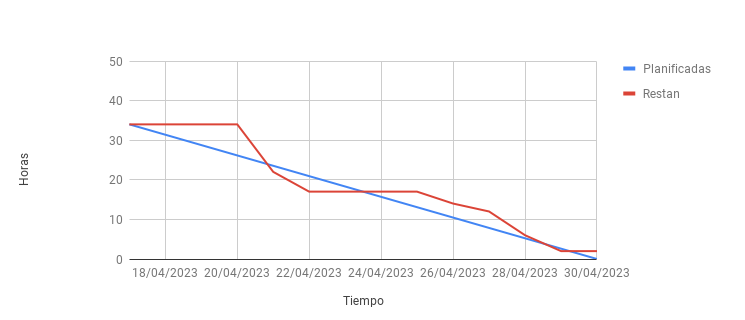
\includegraphics[scale=0.50]{burndown1}
    \caption[Burndown Sprint 1]{Gráfica de la progresión del Burndown en el Sprint 1}
\end{figure}

\section{Sprint 2}

En este segundo sprint se centró el trabajo principalmente en implementar toda la interfaz de usuario que correspondería a la página del editor, incluso si muchas de las funciones accesibles desde este no estaban implementadas. Esto requirió una formación continua a lo largo del sprint en React, tecnología para la que no se contaba experiencia hasta la fecha. Además se implementaría la reproducción de animaciones para los modelos cargados y de audios cargados a la escena. Las historias de usuario incluidas en este sprint son RA-02, RA-04 y RA-05.

\begin{table}[H]
	\resizebox{\textwidth}{!}{%
		\begin{tabular}{|l|l|l|l|l|}
			\hline
			\rowcolor[HTML]{EFEFEF} 
			\textbf{Tarea: TRA-14}           & \textbf{Horas estimadas: 3}      & \textbf{Horas totales: 1}            & \multicolumn{2}{l|}{\cellcolor[HTML]{EFEFEF}\textbf{HU asociada: RA-02}} \\ \hline
			\multicolumn{5}{|l|}{\parbox{12cm}{Hacer diseños de la interfaz de usuario del editor.}}                   \\ \hline
		\end{tabular}%|m{12cm}
	}
\label{TRA-14}
\end{table}

\begin{table}[H]
	\resizebox{\textwidth}{!}{%
		\begin{tabular}{|l|l|l|l|l|}
			\hline
			\rowcolor[HTML]{EFEFEF} 
			\textbf{Tarea: TRA-15}           & \textbf{Horas estimadas: 15}      & \textbf{Horas totales: 14}            & \multicolumn{2}{l|}{\cellcolor[HTML]{EFEFEF}\textbf{HU asociada: RA-02}} \\ \hline
			\multicolumn{5}{|l|}{\parbox{12cm}{Implementar la interfaz de usuario en React}}                   \\ \hline
		\end{tabular}%|m{12cm}
	}
\label{TRA-15}
\end{table}

\begin{table}[H]
	\resizebox{\textwidth}{!}{%
		\begin{tabular}{|l|l|l|l|l|}
			\hline
			\rowcolor[HTML]{EFEFEF} 
			\textbf{Tarea: TRA-16}           & \textbf{Horas estimadas: 2}      & \textbf{Horas totales: 2}            & \multicolumn{2}{l|}{\cellcolor[HTML]{EFEFEF}\textbf{HU asociada: RA-04}} \\ \hline
			\multicolumn{5}{|l|}{\parbox{12cm}{Implementar función que reproduzca una animación en todos los objeto 3D de la escena si es que tienen.}}                   \\ \hline
		\end{tabular}%|m{12cm}
	}
\label{TRA-16}
\end{table}

\begin{table}[H]
	\resizebox{\textwidth}{!}{%
		\begin{tabular}{|l|l|l|l|l|}
			\hline
			\rowcolor[HTML]{EFEFEF} 
			\textbf{Tarea: TRA-17}           & \textbf{Horas estimadas: 1}      & \textbf{Horas totales: 0.5}            & \multicolumn{2}{l|}{\cellcolor[HTML]{EFEFEF}\textbf{HU asociada: RA-05}} \\ \hline
			\multicolumn{5}{|l|}{\parbox{12cm}{Implementar una función que cargue un audio desde un archivo seleccionado desde el navegador de archivos del sistema.}}                   \\ \hline
		\end{tabular}%|m{12cm}
	}
\label{TRA-17}
\end{table}

\begin{table}[H]
	\resizebox{\textwidth}{!}{%
		\begin{tabular}{|l|l|l|l|l|}
			\hline
			\rowcolor[HTML]{EFEFEF} 
			\textbf{Tarea: TRA-18}           & \textbf{Horas estimadas: 1}      & \textbf{Horas totales: 0.5}            & \multicolumn{2}{l|}{\cellcolor[HTML]{EFEFEF}\textbf{HU asociada: RA-05}} \\ \hline
			\multicolumn{5}{|l|}{\parbox{12cm}{Implementar una función que reproduzca el audio cargado de la escena.}}                   \\ \hline
		\end{tabular}%|m{12cm}
	}
\label{TRA-18}
\end{table}

\begin{table}[H]
	\resizebox{\textwidth}{!}{%
		\begin{tabular}{|l|l|l|l|l|}
			\hline
			\rowcolor[HTML]{EFEFEF} 
			\textbf{Tarea: TRA-19}           & \textbf{Horas estimadas: 2}      & \textbf{Horas totales: 4}            & \multicolumn{2}{l|}{\cellcolor[HTML]{EFEFEF}\textbf{HU asociada: RA-02}} \\ \hline
			\multicolumn{5}{|l|}{\parbox{12cm}{Asignar a cada elemento de la interfaz de usuario su funcionalidad correspondiente del editor si es que ya está implementada.}}                   \\ \hline
		\end{tabular}%|m{12cm}
	}
\label{TRA-19}
\end{table}

\begin{table}[H]
	\resizebox{\textwidth}{!}{%
		\begin{tabular}{|l|l|l|l|l|}
			\hline
			\rowcolor[HTML]{EFEFEF} 
			\textbf{Tarea: TRA-20}           & \textbf{Horas estimadas: 2}      & \textbf{Horas totales: 3}            & \multicolumn{2}{l|}{\cellcolor[HTML]{EFEFEF}\textbf{HU asociada: RA-02}} \\ \hline
			\multicolumn{5}{|l|}{\parbox{12cm}{Migrar el código del editor en Three.js a React.}}                   \\ \hline
		\end{tabular}%|m{12cm}
	}
\label{TRA-20}
\end{table}

\begin{table}[H]
	\resizebox{\textwidth}{!}{%
		\begin{tabular}{|l|l|l|l|l|}
			\hline
			\rowcolor[HTML]{EFEFEF} 
			\textbf{Tarea: TRA-21}           & \textbf{Horas estimadas: 1}      & \textbf{Horas totales: 1}            & \multicolumn{2}{l|}{\cellcolor[HTML]{EFEFEF}\textbf{HU asociada: RA-02}} \\ \hline
			\multicolumn{5}{|l|}{\parbox{12cm}{Hacer una página de placeholder que sea la inicial al abrir la aplicación web. Tendrá un único botón que llevará a otra página donde se encuentra el editor.}}                   \\ \hline
		\end{tabular}%|m{12cm}
	}
\label{TRA-21}
\end{table}

Además, durante el transcurso del sprint se añadió una nueva tarea que no se había contemplado al inicio:

\begin{table}[H]
	\resizebox{\textwidth}{!}{%
		\begin{tabular}{|l|l|l|l|l|}
			\hline
			\rowcolor[HTML]{EFEFEF} 
			\textbf{Tarea: TRA-22}           & \textbf{Horas estimadas: 1}      & \textbf{Horas totales: 0.5}            & \multicolumn{2}{l|}{\cellcolor[HTML]{EFEFEF}\textbf{HU asociada: RA-02}} \\ \hline
			\multicolumn{5}{|l|}{\parbox{12cm}{Mudar la lógica de control de la escena de EditorComponent.tsx a una clase Typescript.}}                   \\ \hline
		\end{tabular}%|m{12cm}
	}
\label{TRA-22}
\end{table}

Para comentar el transcurso de este sprint debemos observar antes la gráfica del burndown.

\begin{figure}[h]
    \centering
    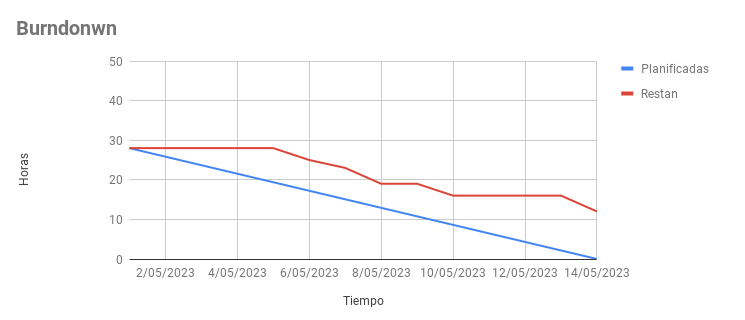
\includegraphics[scale=0.50]{burndown2}
    \caption[Burndown Sprint 2]{Gráfica de la progresión del Burndown en el Sprint 2}
\end{figure}

Como se puede observar, la línea roja del progreso no llega a tocar el eje X de la gráfica, representando que efectivamente quedaron algunas tareas sin completar. Esto se achaca a un problema puntual de salud y de trabajo externo, no a una mala planificación o previsión. Se llega a este razonamiento porque, de las 28 horas planificadas, se realizaron \textbf{24,5 netas y 21,5 reales}. No se habían subestimado las tareas en si, si no el tiempo que se tendría disponible para trabajar en el proyecto durante la franja de la iteración. Independientemente de la razón, el proyecto estaba sufriendo un pequeño retraso, y había que paliarlo de alguna manera. Como opciones se presentaban alargar algunos días el sprint, o pasar las tareas sin completar a la siguiente iteración. Se optó por esto último. Las tareas TRA-21 y TRA-16 se terminarían en el Sprint 3.

\section{Sprint 3}

Este sprint orbitó alrededor del desarrollo de las funcionalidades básicas para la app Android. Se pretendía tener funcionales los tres tipos de escenas en esta. Además se implementaría la opción de exportar y descargar escenas desde el editor web. Por último se completarían las tareas atrasadas del sprint anterior. Las historias que describen este sprint son  RA-13, RA-11.1, RA-11.2, RA-11.3.

\begin{table}[H]
	\resizebox{\textwidth}{!}{%
		\begin{tabular}{|l|l|l|l|l|}
			\hline
			\rowcolor[HTML]{EFEFEF} 
			\textbf{Tarea: TRA-22b}           & \textbf{Horas estimadas: 0.5}      & \textbf{Horas totales: 0.5}            & \multicolumn{2}{l|}{\cellcolor[HTML]{EFEFEF}\textbf{HUs RA-11.1 RA-11.2 RA-11.3}} \\ \hline
			\multicolumn{5}{|l|}{\parbox{12cm}{Realizar configuración inicial del proyecto de Android Studio.}}                   \\ \hline
		\end{tabular}%|m{12cm}
	}
\label{TRA-22b}
\end{table}

\begin{table}[H]
	\resizebox{\textwidth}{!}{%
		\begin{tabular}{|l|l|l|l|l|}
			\hline
			\rowcolor[HTML]{EFEFEF} 
			\textbf{Tarea: TRA-23}           & \textbf{Horas estimadas: 2}      & \textbf{Horas totales: 0.5}            & \multicolumn{2}{l|}{\cellcolor[HTML]{EFEFEF}\textbf{HUs RA-11.1 RA-11.2 RA-11.3}} \\ \hline
			\multicolumn{5}{|l|}{\parbox{12cm}{Implementar reproducción de sonidos en la app de Android Studio.}}                   \\ \hline
		\end{tabular}%|m{12cm}
	}
\label{TRA-23}
\end{table}

\begin{table}[H]
	\resizebox{\textwidth}{!}{%
		\begin{tabular}{|l|l|l|l|l|}
			\hline
			\rowcolor[HTML]{EFEFEF} 
			\textbf{Tarea: TRA-24}           & \textbf{Horas estimadas: 2}      & \textbf{Horas totales: 2}            & \multicolumn{2}{l|}{\cellcolor[HTML]{EFEFEF}\textbf{HUs RA-11.1 RA-11.2 RA-11.3}} \\ \hline
			\multicolumn{5}{|l|}{\parbox{12cm}{Implementar escena AR de ejemplo de la documentación de Sceneview.}}                   \\ \hline
		\end{tabular}%|m{12cm}
	}
\label{TRA-24}
\end{table}

\begin{table}[H]
	\resizebox{\textwidth}{!}{%
		\begin{tabular}{|l|l|l|l|l|}
			\hline
			\rowcolor[HTML]{EFEFEF} 
			\textbf{Tarea: TRA-25}           & \textbf{Horas estimadas: 3}      & \textbf{Horas totales: 2}            & \multicolumn{2}{l|}{\cellcolor[HTML]{EFEFEF}\textbf{HU asociada RA-11.1}} \\ \hline
			\multicolumn{5}{|l|}{\parbox{12cm}{Implementar modo de escenas por marcador en la app Android siguiendo el ejemplo de la documentación.}}                   \\ \hline
		\end{tabular}%|m{12cm}
	}
\label{TRA-25}
\end{table}

\begin{table}[H]
	\resizebox{\textwidth}{!}{%
		\begin{tabular}{|l|l|l|l|l|}
			\hline
			\rowcolor[HTML]{EFEFEF} 
			\textbf{Tarea: TRA-26}           & \textbf{Horas estimadas: 3}      & \textbf{Horas totales: 3}            & \multicolumn{2}{l|}{\cellcolor[HTML]{EFEFEF}\textbf{HU asociada RA-11.3}} \\ \hline
			\multicolumn{5}{|l|}{\parbox{12cm}{Implementar modo de escenas geoespaciales en la app Android siguiendo el ejemplo de la documentación.}}                   \\ \hline
		\end{tabular}%|m{12cm}
	}
\label{TRA-26}
\end{table}

\begin{table}[H]
	\resizebox{\textwidth}{!}{%
		\begin{tabular}{|l|l|l|l|l|}
			\hline
			\rowcolor[HTML]{EFEFEF} 
			\textbf{Tarea: TRA-27}           & \textbf{Horas estimadas: 3}      & \textbf{Horas totales: 2}            & \multicolumn{2}{l|}{\cellcolor[HTML]{EFEFEF}\textbf{HU asociada RA-11.2}} \\ \hline
			\multicolumn{5}{|l|}{\parbox{12cm}{Implementar modo de escenas de posicionamiento sobre superficies en la app Android siguiendo el ejemplo de la documentación.}}                   \\ \hline
		\end{tabular}%|m{12cm}
	}
\label{TRA-27}
\end{table}

\begin{table}[H]
	\resizebox{\textwidth}{!}{%
		\begin{tabular}{|l|l|l|l|l|}
			\hline
			\rowcolor[HTML]{EFEFEF} 
			\textbf{Tarea: TRA-28}           & \textbf{Horas estimadas: 2}      & \textbf{Horas totales: 0.5}            & \multicolumn{2}{l|}{\cellcolor[HTML]{EFEFEF}\textbf{HUs RA-11.1 RA-11.2 RA-11.3}} \\ \hline
			\multicolumn{5}{|l|}{\parbox{12cm}{Implementar la reproducción de animaciones para los modelos en caso de que estos tengan y así se especifique en el JSON de entrada.}}                   \\ \hline
		\end{tabular}%|m{12cm}
	}
\label{TRA-28}
\end{table}

\begin{table}[H]
	\resizebox{\textwidth}{!}{%
		\begin{tabular}{|l|l|l|l|l|}
			\hline
			\rowcolor[HTML]{EFEFEF} 
			\textbf{Tarea: TRA-29}           & \textbf{Horas estimadas: 8}      & \textbf{Horas totales: 6}            & \multicolumn{2}{l|}{\cellcolor[HTML]{EFEFEF}\textbf{HU asociada RA-13}} \\ \hline
			\multicolumn{5}{|l|}{\parbox{12cm}{Implementar una función que exporte todos los modelos de la escena a un solo modelo glb y lo descargue.}}                   \\ \hline
		\end{tabular}%|m{12cm}
	}
\label{TRA-29}
\end{table}

\begin{table}[H]
	\resizebox{\textwidth}{!}{%
		\begin{tabular}{|l|l|l|l|l|}
			\hline
			\rowcolor[HTML]{EFEFEF} 
			\textbf{Tarea: TRA-30}           & \textbf{Horas estimadas: 0.5}      & \textbf{Horas totales: 1}            & \multicolumn{2}{l|}{\cellcolor[HTML]{EFEFEF}\textbf{HU asociada RA-13}} \\ \hline
			\multicolumn{5}{|l|}{\parbox{12cm}{Diseñar un archivo JSON  para la salida del editor y la entrada de la app. Este deberá indicar los parámetros necesarios para la configuración de una escena, como el tipo de la misma, si tiene audio o animaciones, sus modelos, etc.}}                   \\ \hline
		\end{tabular}%|m{12cm}
	}
\label{TRA-30}
\end{table}

\begin{figure}[h]
    \centering
    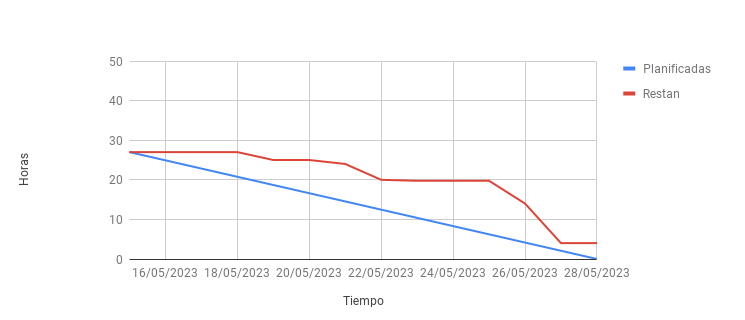
\includegraphics[scale=0.50]{burndown3}
    \caption[Burndown Sprint 3]{Gráfica de la progresión del Burndown en el Sprint 3}
\end{figure}

En esta iteración se cumplieron la mayoría de los objetivos que se propusieran. La funcionalidad básica de la app Android estaba completa, pero la TRA-29 se había quedado a medias de la implementación. Era un retraso bastante mínimo así que se decidió pasar lo que restaba de la tarea al siguiente sprint de nuevo.

\section{Sprint 4}

Esta iteración se implementarían las funcionalidades de cuentas de usuario e inicio de sesión, y para ello habría que desarrollar un backend al que pudieran conectarse tanto el editor web como la app y hacer las llamadas que necesitaran a la API para operaciones como crear un usuario o actualizar una escena. Sin embargo, a lo largo de la formación que se realizó en estas tecnologías y antes de redactar las tareas de la iteración, se llegó a la conclusión que se necesitaba más tiempo de desarrollo para implementarlo que lo que se había planeado para este sprint. Sobre todo ocurría que con todo el código que había que preparar tanto en el backend como en el frontend para conectar ambos, a penas daba tiempo a implementar correctamente las interfaces de usuario que se requerían. Además había que recuperar un pequeño retraso del sprint anterior.

Esto no supuso ningún golpe para el proyecto, ya que se anticipó una posible situación similar. El area en el que menos experiencia se tenía a la hora de comenzar el desarrollo era en el desarrollo de backend. Y aunque se hicieron estimaciones, se contemplaba la posibilidad de que pudieran ser erroneas desde un inicio. Es por ello que para el sprint 5 se designaron las historias de usuario de menor prioridad de las cuales podía prescindir el proyecto si se diera el caso como la creación de figuras básicas, la filtración de escenas o las múltiples imágenes activadoras en imágenes aumentadas. Por tanto se tomó la decisión de descartar esas historias y re organizar el Sprint 5. En el 4 se realizaron las siguientes tareas.

\begin{table}[H]
	\resizebox{\textwidth}{!}{%
		\begin{tabular}{|l|l|l|l|l|}
			\hline
			\rowcolor[HTML]{EFEFEF} 
			\textbf{Tarea: TRA-31}           & \textbf{Horas estimadas: 1}      & \textbf{Horas totales: 2}            & \multicolumn{2}{l|}{\cellcolor[HTML]{EFEFEF}\textbf{HU asociada RA-10}} \\ \hline
			\multicolumn{5}{|l|}{\parbox{12cm}{Crear proyecto base de Node.js con Express.}}                   \\ \hline
		\end{tabular}%|m{12cm}
	}
\label{TRA-31}
\end{table}

\begin{table}[H]
	\resizebox{\textwidth}{!}{%
		\begin{tabular}{|l|l|l|l|l|}
			\hline
			\rowcolor[HTML]{EFEFEF} 
			\textbf{Tarea: TRA-32}           & \textbf{Horas estimadas: 1}      & \textbf{Horas totales: 1}            & \multicolumn{2}{l|}{\cellcolor[HTML]{EFEFEF}\textbf{HU asociada RA-10}} \\ \hline
			\multicolumn{5}{|l|}{\parbox{12cm}{Crear y configurar proyecto de Google Firebase, obteniendo las claves secretas necesarias e incluyéndolas en el proyecto de Node.js.}}                   \\ \hline
		\end{tabular}%|m{12cm}
	}
\label{TRA-32}
\end{table}

\begin{table}[H]
	\resizebox{\textwidth}{!}{%
		\begin{tabular}{|l|l|l|l|l|}
			\hline
			\rowcolor[HTML]{EFEFEF} 
			\textbf{Tarea: TRA-33}           & \textbf{Horas estimadas: 1}      & \textbf{Horas totales: -}            & \multicolumn{2}{l|}{\cellcolor[HTML]{EFEFEF}\textbf{HU asociada RA-10}} \\ \hline
			\multicolumn{5}{|l|}{\parbox{12cm}{Implementar función en Node.js para el inicio de sesión de un usuario.}}                   \\ \hline
		\end{tabular}%|m{12cm}
	}
\label{TRA-33}
\end{table}


\begin{table}[H]
	\resizebox{\textwidth}{!}{%
		\begin{tabular}{|l|l|l|l|l|}
			\hline
			\rowcolor[HTML]{EFEFEF} 
			\textbf{Tarea: TRA-34}           & \textbf{Horas estimadas: 1}      & \textbf{Horas totales: -}            & \multicolumn{2}{l|}{\cellcolor[HTML]{EFEFEF}\textbf{HU asociada RA-10}} \\ \hline
			\multicolumn{5}{|l|}{\parbox{12cm}{Implementar función en Node.js para la creación de una cuenta de usuario.}}                   \\ \hline
		\end{tabular}%|m{12cm}
	}
\label{TRA-34}
\end{table}

\begin{table}[H]
	\resizebox{\textwidth}{!}{%
		\begin{tabular}{|l|l|l|l|l|}
			\hline
			\rowcolor[HTML]{EFEFEF} 
			\textbf{Tarea: TRA-35}           & \textbf{Horas estimadas: 1}      & \textbf{Horas totales: 1}            & \multicolumn{2}{l|}{\cellcolor[HTML]{EFEFEF}\textbf{HU asociada RA-10.2}} \\ \hline
			\multicolumn{5}{|l|}{\parbox{12cm}{Implementar función en Node.js para la creación de una nueva escena.}}                   \\ \hline
		\end{tabular}%|m{12cm}
	}
\label{TRA-35}
\end{table}

\begin{table}[H]
	\resizebox{\textwidth}{!}{%
		\begin{tabular}{|l|l|l|l|l|}
			\hline
			\rowcolor[HTML]{EFEFEF} 
			\textbf{Tarea: TRA-36}           & \textbf{Horas estimadas: 1}      & \textbf{Horas totales: 1}            & \multicolumn{2}{l|}{\cellcolor[HTML]{EFEFEF}\textbf{HU asociada RA-10.2}} \\ \hline
			\multicolumn{5}{|l|}{\parbox{12cm}{Implementar función en Node.js para eliminar una escena a partir de su identificador.}}                   \\ \hline
		\end{tabular}%|m{12cm}
	}
\label{TRA-36}
\end{table}

\begin{table}[H]
	\resizebox{\textwidth}{!}{%
		\begin{tabular}{|l|l|l|l|l|}
			\hline
			\rowcolor[HTML]{EFEFEF} 
			\textbf{Tarea: TRA-37}           & \textbf{Horas estimadas: 1}      & \textbf{Horas totales: 1}            & \multicolumn{2}{l|}{\cellcolor[HTML]{EFEFEF}\textbf{HU asociada RA-10.2}} \\ \hline
			\multicolumn{5}{|l|}{\parbox{12cm}{Implementar función en Node.js para actualizar una escena ya existente.}}                   \\ \hline
		\end{tabular}%|m{12cm}
	}
\label{TRA-37}
\end{table}

\begin{table}[H]
	\resizebox{\textwidth}{!}{%
		\begin{tabular}{|l|l|l|l|l|}
			\hline
			\rowcolor[HTML]{EFEFEF} 
			\textbf{Tarea: TRA-38}           & \textbf{Horas estimadas: 1}      & \textbf{Horas totales: 1}            & \multicolumn{2}{l|}{\cellcolor[HTML]{EFEFEF}\textbf{HU asociada RA-10.2}} \\ \hline
			\multicolumn{5}{|l|}{\parbox{12cm}{Implementar función en Node.js para obtener todas las escenas de un usuario concreto.}}                   \\ \hline
		\end{tabular}%|m{12cm}
	}
\label{TRA-38}
\end{table}

\begin{table}[H]
	\resizebox{\textwidth}{!}{%
		\begin{tabular}{|l|l|l|l|l|}
			\hline
			\rowcolor[HTML]{EFEFEF} 
			\textbf{Tarea: TRA-39}           & \textbf{Horas estimadas: 1}      & \textbf{Horas totales: 2}            & \multicolumn{2}{l|}{\cellcolor[HTML]{EFEFEF}\textbf{HU asociada RA-10.2}} \\ \hline
			\multicolumn{5}{|l|}{\parbox{12cm}{Configurar Firebase Storage para poder almacenar objetos binarios como imágenes o modelos 3D y que sean accesibles desde una url para descargarlos.}}                   \\ \hline
		\end{tabular}%|m{12cm}
	}
\label{TRA-39}
\end{table}

\begin{table}[H]
	\resizebox{\textwidth}{!}{%
		\begin{tabular}{|l|l|l|l|l|}
			\hline
			\rowcolor[HTML]{EFEFEF} 
			\textbf{Tarea: TRA-40}           & \textbf{Horas estimadas: 1}      & \textbf{Horas totales: 1}            & \multicolumn{2}{l|}{\cellcolor[HTML]{EFEFEF}\textbf{HU asociada RA-10.2}} \\ \hline
			\multicolumn{5}{|l|}{\parbox{12cm}{Diseñar las tablas de bases de datos para usuarios y escenas.}}                   \\ \hline
		\end{tabular}%|m{12cm}
	}
\label{TRA-40}
\end{table}

\begin{table}[H]
	\resizebox{\textwidth}{!}{%
		\begin{tabular}{|l|l|l|l|l|}
			\hline
			\rowcolor[HTML]{EFEFEF} 
			\textbf{Tarea: TRA-41}           & \textbf{Horas estimadas: 2}      & \textbf{Horas totales: 2}            & \multicolumn{2}{l|}{\cellcolor[HTML]{EFEFEF}\textbf{HU asociada RA-10.2}} \\ \hline
			\multicolumn{5}{|l|}{\parbox{12cm}{Implementar las tablas de bases de datos en Google Firebase.}}                   \\ \hline
		\end{tabular}%|m{12cm}
	}
\label{TRA-41}
\end{table}

\begin{table}[H]
	\resizebox{\textwidth}{!}{%
		\begin{tabular}{|l|l|l|l|l|}
			\hline
			\rowcolor[HTML]{EFEFEF} 
			\textbf{Tarea: TRA-42}           & \textbf{Horas estimadas: 2}      & \textbf{Horas totales: 2}            & \multicolumn{2}{l|}{\cellcolor[HTML]{EFEFEF}\textbf{HU asociada RA-12}} \\ \hline
			\multicolumn{5}{|l|}{\parbox{12cm}{Configurar acceso a Firebase Storage desde la app Android.}}                   \\ \hline
		\end{tabular}%|m{12cm}
	}
\label{TRA-42}
\end{table}

\begin{table}[H]
	\resizebox{\textwidth}{!}{%
		\begin{tabular}{|l|l|l|l|l|}
			\hline
			\rowcolor[HTML]{EFEFEF} 
			\textbf{Tarea: TRA-43}           & \textbf{Horas estimadas: 10}      & \textbf{Horas totales: 8}            & \multicolumn{2}{l|}{\cellcolor[HTML]{EFEFEF}\textbf{HU asociada RA-10}} \\ \hline
			\multicolumn{5}{|l|}{\parbox{12cm}{Configurar acceso a Firebase Storage y API desde React. Asignar a cada menú de la aplicación su llamada correspondiente.}}                   \\ \hline
		\end{tabular}%|m{12cm}
	}
\label{TRA-43}
\end{table}

\begin{table}[H]
	\resizebox{\textwidth}{!}{%
		\begin{tabular}{|l|l|l|l|l|}
			\hline
			\rowcolor[HTML]{EFEFEF} 
			\textbf{Tarea: TRA-44}           & \textbf{Horas estimadas: 1}      & \textbf{Horas totales: -}            & \multicolumn{2}{l|}{\cellcolor[HTML]{EFEFEF}\textbf{HU asociada RA-10}} \\ \hline
			\multicolumn{5}{|l|}{\parbox{12cm}{Implementar función en Node.js para la modificación de datos de un usuario.}}                   \\ \hline
		\end{tabular}%|m{12cm}
	}
\label{TRA-44}
\end{table}

\begin{table}[H]
	\resizebox{\textwidth}{!}{%
		\begin{tabular}{|l|l|l|l|l|}
			\hline
			\rowcolor[HTML]{EFEFEF} 
			\textbf{Tarea: TRA-45}           & \textbf{Horas estimadas: 1}      & \textbf{Horas totales: -}            & \multicolumn{2}{l|}{\cellcolor[HTML]{EFEFEF}\textbf{HU asociada RA-10}} \\ \hline
			\multicolumn{5}{|l|}{\parbox{12cm}{Implementar función en Node.js para la eliminación de un usuario.}}                   \\ \hline
		\end{tabular}%|m{12cm}
	}
\label{TRA-45}
\end{table}

Algo importante a destacar en este Sprint es que las tareas TRA-33, TRA-34, TRA-44 y TRA-45 fueron descartadas durante el desarrollo. Esto se debe a que, como se comentará en el capítulo de Implementación, se decidió optar por otra vía en cuanto a la gestión de cuentas de usuario se refiere, por lo que ya no sería necesario crear estas llamadas en la API. En esta iteración se dispuso de más tiempo, lo cual se reflejó en la compleción de todas las tareas a tiempo.

\begin{figure}[h]
    \centering
    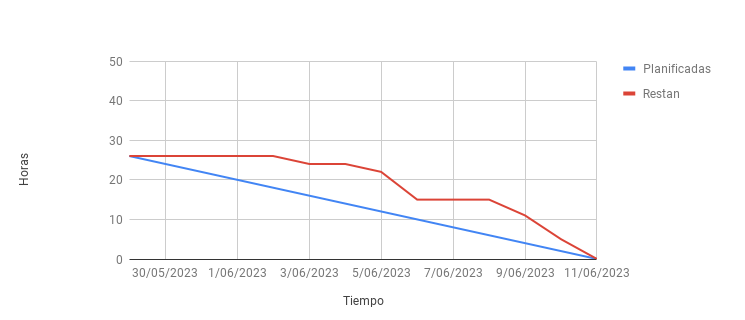
\includegraphics[scale=0.50]{burndown4}
    \caption[Burndown Sprint 4]{Gráfica de la progresión del Burndown en el Sprint 4}
\end{figure}

\section{Sprint 5}

Este sprint en un inicio se planificó como un colchón en caso de que la planificación no fuera al ritmo esperado en el resto de sprints. Se desarrollarían las historias RA-9, RA-9.1, RA-12.2 y RA-3, de prioridad LOW, sin las cuales el sistema podía existir sin perder demasiado. Como ya se comentó en anteriores sprints, se descartó la implementación de todas ellas, y en su lugar se continuó con RA-10, RA-10.2 y RA-12 del cuarto sprint, que requerían de más tiempo además de RA-10.1 y RA-12.1 de prioridad MID que sí estaban programadas para esta iteración.

\begin{table}[H]
	\resizebox{\textwidth}{!}{%
		\begin{tabular}{|l|l|l|l|l|}
			\hline
			\rowcolor[HTML]{EFEFEF} 
			\textbf{Tarea: TRA-47}           & \textbf{Horas estimadas: 4}      & \textbf{Horas totales: 4}            & \multicolumn{2}{l|}{\cellcolor[HTML]{EFEFEF}\textbf{HU asociada RA-12.1}} \\ \hline
			\multicolumn{5}{|l|}{\parbox{12cm}{Implementar menú de selección de escena en la aplicación Android.}}                   \\ \hline
		\end{tabular}%|m{12cm}
	}
\label{TRA-47}
\end{table}

\begin{table}[H]
	\resizebox{\textwidth}{!}{%
		\begin{tabular}{|l|l|l|l|l|}
			\hline
			\rowcolor[HTML]{EFEFEF} 
			\textbf{Tarea: TRA-48}           & \textbf{Horas estimadas: 4}      & \textbf{Horas totales: 4}            & \multicolumn{2}{l|}{\cellcolor[HTML]{EFEFEF}\textbf{HU asociada RA-10.1}} \\ \hline
			\multicolumn{5}{|l|}{\parbox{12cm}{Implementar menú de selección de escena la aplicación web.}}                   \\ \hline
		\end{tabular}%|m{12cm}
	}
\label{TRA-48}
\end{table}

\begin{table}[H]
	\resizebox{\textwidth}{!}{%
		\begin{tabular}{|l|l|l|l|l|}
			\hline
			\rowcolor[HTML]{EFEFEF} 
			\textbf{Tarea: TRA-49}           & \textbf{Horas estimadas: 2}      & \textbf{Horas totales: 4}            & \multicolumn{2}{l|}{\cellcolor[HTML]{EFEFEF}\textbf{HU asociada RA-12.1}} \\ \hline
			\multicolumn{5}{|l|}{\parbox{12cm}{Configurar la API de acceso al backend para que sea accesible desde otros dispositivos de la red.}}                   \\ \hline
		\end{tabular}%|m{12cm}
	}
\label{TRA-49}
\end{table}

\begin{table}[H]
	\resizebox{\textwidth}{!}{%
		\begin{tabular}{|l|l|l|l|l|}
			\hline
			\rowcolor[HTML]{EFEFEF} 
			\textbf{Tarea: TRA-50}           & \textbf{Horas estimadas: 3}      & \textbf{Horas totales: 3}            & \multicolumn{2}{l|}{\cellcolor[HTML]{EFEFEF}\textbf{HU asociada RA-10}} \\ \hline
			\multicolumn{5}{|l|}{\parbox{12cm}{Implementar funciones para el inicio de sesión y registro de un usuario a partir de un correo y contraseña en la aplicación web.}}                   \\ \hline
		\end{tabular}%|m{12cm}
	}
\label{TRA-50}
\end{table}

\begin{table}[H]
	\resizebox{\textwidth}{!}{%
		\begin{tabular}{|l|l|l|l|l|}
			\hline
			\rowcolor[HTML]{EFEFEF} 
			\textbf{Tarea: TRA-51}           & \textbf{Horas estimadas: 2}      & \textbf{Horas totales: 2}            & \multicolumn{2}{l|}{\cellcolor[HTML]{EFEFEF}\textbf{HU asociada RA-12}} \\ \hline
			\multicolumn{5}{|l|}{\parbox{12cm}{Implementar inicio de sesión con usuario y contraseña en la aplicación Android.}}                   \\ \hline
		\end{tabular}%|m{12cm}
	}
\label{TRA-53}
\end{table}

\begin{table}[H]
	\resizebox{\textwidth}{!}{%
		\begin{tabular}{|l|l|l|l|l|}
			\hline
			\rowcolor[HTML]{EFEFEF} 
			\textbf{Tarea: TRA-53}           & \textbf{Horas estimadas: 2}      & \textbf{Horas totales: 4}            & \multicolumn{2}{l|}{\cellcolor[HTML]{EFEFEF}\textbf{HU asociada RA-12.1}} \\ \hline
			\multicolumn{5}{|l|}{\parbox{12cm}{Implementar petición GET desde la app Android a la API para obtener las escenas creadas por un usuario.}}                   \\ \hline
		\end{tabular}%|m{12cm}
	}
\label{TRA-53}
\end{table}

\begin{table}[H]
	\resizebox{\textwidth}{!}{%
		\begin{tabular}{|l|l|l|l|l|}
			\hline
			\rowcolor[HTML]{EFEFEF} 
			\textbf{Tarea: TRA-55}           & \textbf{Horas estimadas: 1}      & \textbf{Horas totales: 1}            & \multicolumn{2}{l|}{\cellcolor[HTML]{EFEFEF}\textbf{HU asociada RA-10.1}} \\ \hline
			\multicolumn{5}{|l|}{\parbox{12cm}{Implementar menú para el cambio de credenciales de un usuario en el editor web.}}                   \\ \hline
		\end{tabular}%|m{12cm}
	}
\label{TRA-55}
\end{table}

\begin{table}[H]
	\resizebox{\textwidth}{!}{%
		\begin{tabular}{|l|l|l|l|l|}
			\hline
			\rowcolor[HTML]{EFEFEF} 
			\textbf{Tarea: TRA-56}           & \textbf{Horas estimadas: 3}      & \textbf{Horas totales: 3}            & \multicolumn{2}{l|}{\cellcolor[HTML]{EFEFEF}\textbf{HU asociada RA-10}} \\ \hline
			\multicolumn{5}{|l|}{\parbox{12cm}{Proteger las rutas que no sean la página de login del editor web para solo poder acceder a ellas cuando hay una sesión iniciada.}}                   \\ \hline
		\end{tabular}%|m{12cm}
	}
\label{TRA-56}
\end{table}

\begin{table}[H]
	\resizebox{\textwidth}{!}{%
		\begin{tabular}{|l|l|l|l|l|}
			\hline
			\rowcolor[HTML]{EFEFEF} 
			\textbf{Tarea: TRA-57}           & \textbf{Horas estimadas: 10}      & \textbf{Horas totales: 7}            & \multicolumn{2}{l|}{\cellcolor[HTML]{EFEFEF}\textbf{HU asociada RA-10.2}} \\ \hline
			\multicolumn{5}{|l|}{\parbox{12cm}{Implementar la carga, guardado y borrado de una escena a partir del JSON obtenido por la API con Firebase Storage en el editor web.}}                   \\ \hline
		\end{tabular}%|m{12cm}
	}
\label{TRA-57}
\end{table}

\begin{table}[H]
	\resizebox{\textwidth}{!}{%
		\begin{tabular}{|l|l|l|l|l|}
			\hline
			\rowcolor[HTML]{EFEFEF} 
			\textbf{Tarea: TRA-58}           & \textbf{Horas estimadas: 2}      & \textbf{Horas totales: 1.5}            & \multicolumn{2}{l|}{\cellcolor[HTML]{EFEFEF}\textbf{HU asociada RA-10.2}} \\ \hline
			\multicolumn{5}{|l|}{\parbox{12cm}{Añadir animación de carga para momentos en los que se esté esperando la respuesta a una petición o la carga de algún recurso desde el editor web.}}                   \\ \hline
		\end{tabular}%|m{12cm}
	}
\label{TRA-58}
\end{table}

\begin{table}[H]
	\resizebox{\textwidth}{!}{%
		\begin{tabular}{|l|l|l|l|l|}
			\hline
			\rowcolor[HTML]{EFEFEF} 
			\textbf{Tarea: TRA-59}           & \textbf{Horas estimadas: 3}      & \textbf{Horas totales: 2}            & \multicolumn{2}{l|}{\cellcolor[HTML]{EFEFEF}\textbf{HU asociada RA-10.2}} \\ \hline
			\multicolumn{5}{|l|}{\parbox{12cm}{Implementar menús pop-up de confirmación  para las acciones de eliminar una escena, abandonar el editor y cerrar sesión desde el editor web.}}                   \\ \hline
		\end{tabular}%|m{12cm}
	}
\label{TRA-59}
\end{table}

El sprint finalizó sin mayores complicaciones, teniendo el producto final listo. A estas alturas se notó la experiencia obtenida en el proceso de planificación, el cual fue preciso. Una vez terminado el producto solo restaba desplegar la aplicación.

\begin{figure}[h]
    \centering
    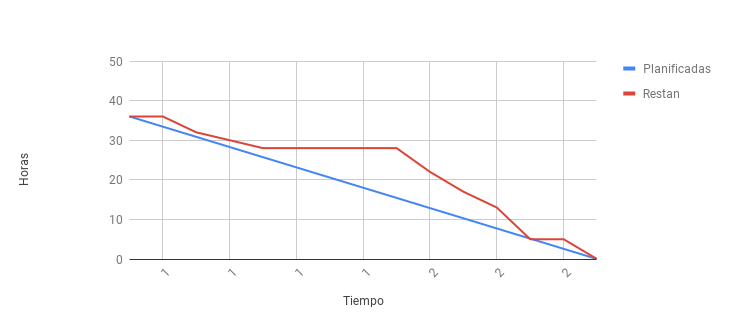
\includegraphics[scale=0.50]{burndown5}
    \caption[Burndown Sprint 5]{Gráfica de la progresión del Burndown en el Sprint 5}
\end{figure}